\subsection{Sequentially consistent IVL priority queue}
\label{ivl-ssec:priority-q}

We next show that for more complex (non-numeric) objects, IVL can be used in conjuction
with additional properties.
Consider the example of a \emph{Priority Queue (PQ)}, which supports two operations, \textsc{insert}
and \textsc{deleteMin}~\cite{van1976design, ronngren1997comparative}.
The sequential PQ holds a set of priority-element pairs.
An \textsc{insert}$(e,p)$ adds element $e$ with priority $p$ to the set,
and a \textsc{deleteMin} returns and removes the element with the lowest priority
from the set.

The set of pairs is partially ordered by priority, with ties broken
by the elements themselves.
Thus, we can use IVL to define the PQ's concurrent semantics.
However, IVL alone allows the PQ to return
elements that were never inserted, as shown in Figure~\ref{ivl-fig:PQ-IVL-not-SC}. In the example, thread $p_1$
inserts $(e_1,8)$ to the PQ and thread $p_2$ inserts $(e_2,3)$. Concurrently to the insertions, thread
$q$ removes an item from the PQ. IVL allows $q$ to return $(e_x,6)$, as $(e_2,3) \leq (e_x,6) \leq (e_2,8)$,
even though $(e_x,6)$ may be an element that was never inserted to the PQ.
Thus, an IVL PQ is meaningless. Fortunately, we can address this by requiring an additional
property along with IVL.

To disallow such spurious elements, we require that the PQ also be \emph{sequentially
consistent (SC)}~\cite{scheurich1987correct}. We note that SC and IVL are incomparable: IVL requires that sequential
executions adhere to the sequential specification, whereas SC only requires program order. For example,
Figure~\ref{ivl-fig:SC-IVL-not-IVL} shows an SC PQ that isn't IVL, and, as noted above, Figure~\ref{ivl-fig:PQ-IVL-not-SC}
shows an IVL PQ that isn't SC.

\begin{figure}[htb]
  \begin{subfigure}[b]{.45\linewidth}
      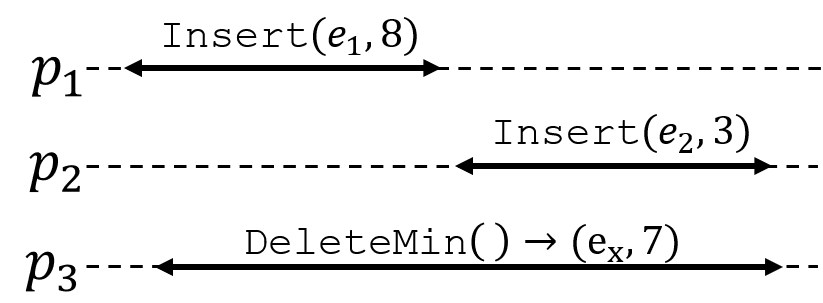
\includegraphics[width=0.32\textwidth]{graphics/ivl/PQIVLnotSC.png}
  \caption{IVL PQ that isn't SC -- $(e_x,7)$ is returned even though it was never inserted.}
  \label{ivl-fig:PQ-IVL-not-SC}
  \end{subfigure}
  \begin{subfigure}[b]{.55\linewidth}
    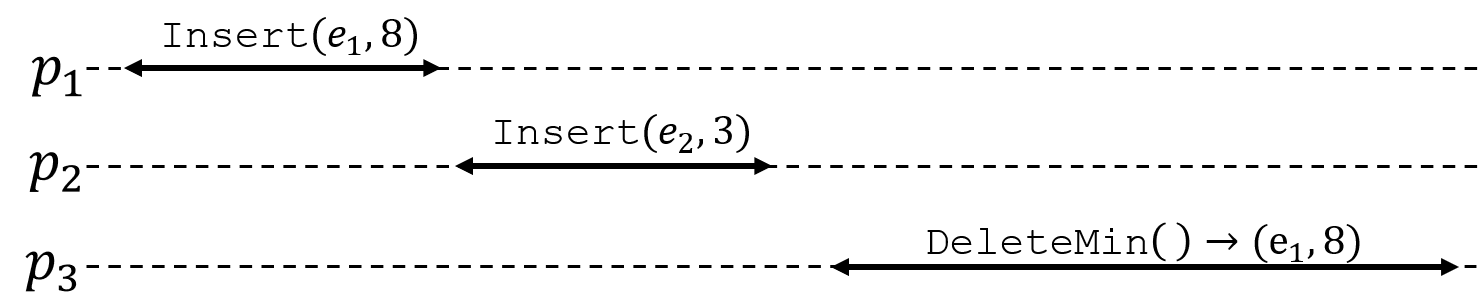
\includegraphics[width={0.58\textwidth}]{graphics/ivl/PQSCnotIVL.png}
  \caption{SC PQ that isn't IVL -- IVL adheres to real-time order, therefore $(e_2,3)$ must be returned.}
  \label{ivl-fig:SC-IVL-not-IVL}
  \end{subfigure}
  \caption{Possible histories of a priority queue under IVL only (\ref{ivl-fig:PQ-IVL-not-SC}) and SC only (\ref{ivl-fig:SC-IVL-not-IVL}).}
\end{figure}

Combining the IVL and SC properties yields a PQ that must return elements previously inserted
to the PQ and not yet deleted (by SC), yet the \textsc{deleteMin} operation may return elements
disallowed under linearizability. For example, Figure~\ref{ivl-fig:SC-IVL-and-SC} presents
a history of an IVL and SC PQ. In the
example, thread $p_1$ inserts $(e_1,8)$ to the PQ, $p_2$ then inserts $(e_2,3)$, and
then $p_1$ inserts $(e_3, 5)$. Concurrently to the insertions, $p_3$ removes an element
from the PQ. The SC property requires that the element be $(e_1,8)$, $(e_2,3)$ or $(e_3,5)$,
and the IVL property requires that the element have priority at most $8$, and at least $3$.
For example, the element $(e_3, 5)$ can be returned, which is disallowed under linearizability.

An IVL priority queue is useful when the necessary guarantee is that the popped element is one of the
top elements, but not necessarily the top one, e.g., parallel graph processing~\cite{gonzalez2012powergraph},
or belief propagation~\cite{aksenov2020scalable}.

\begin{figure}[b]
  \centering
  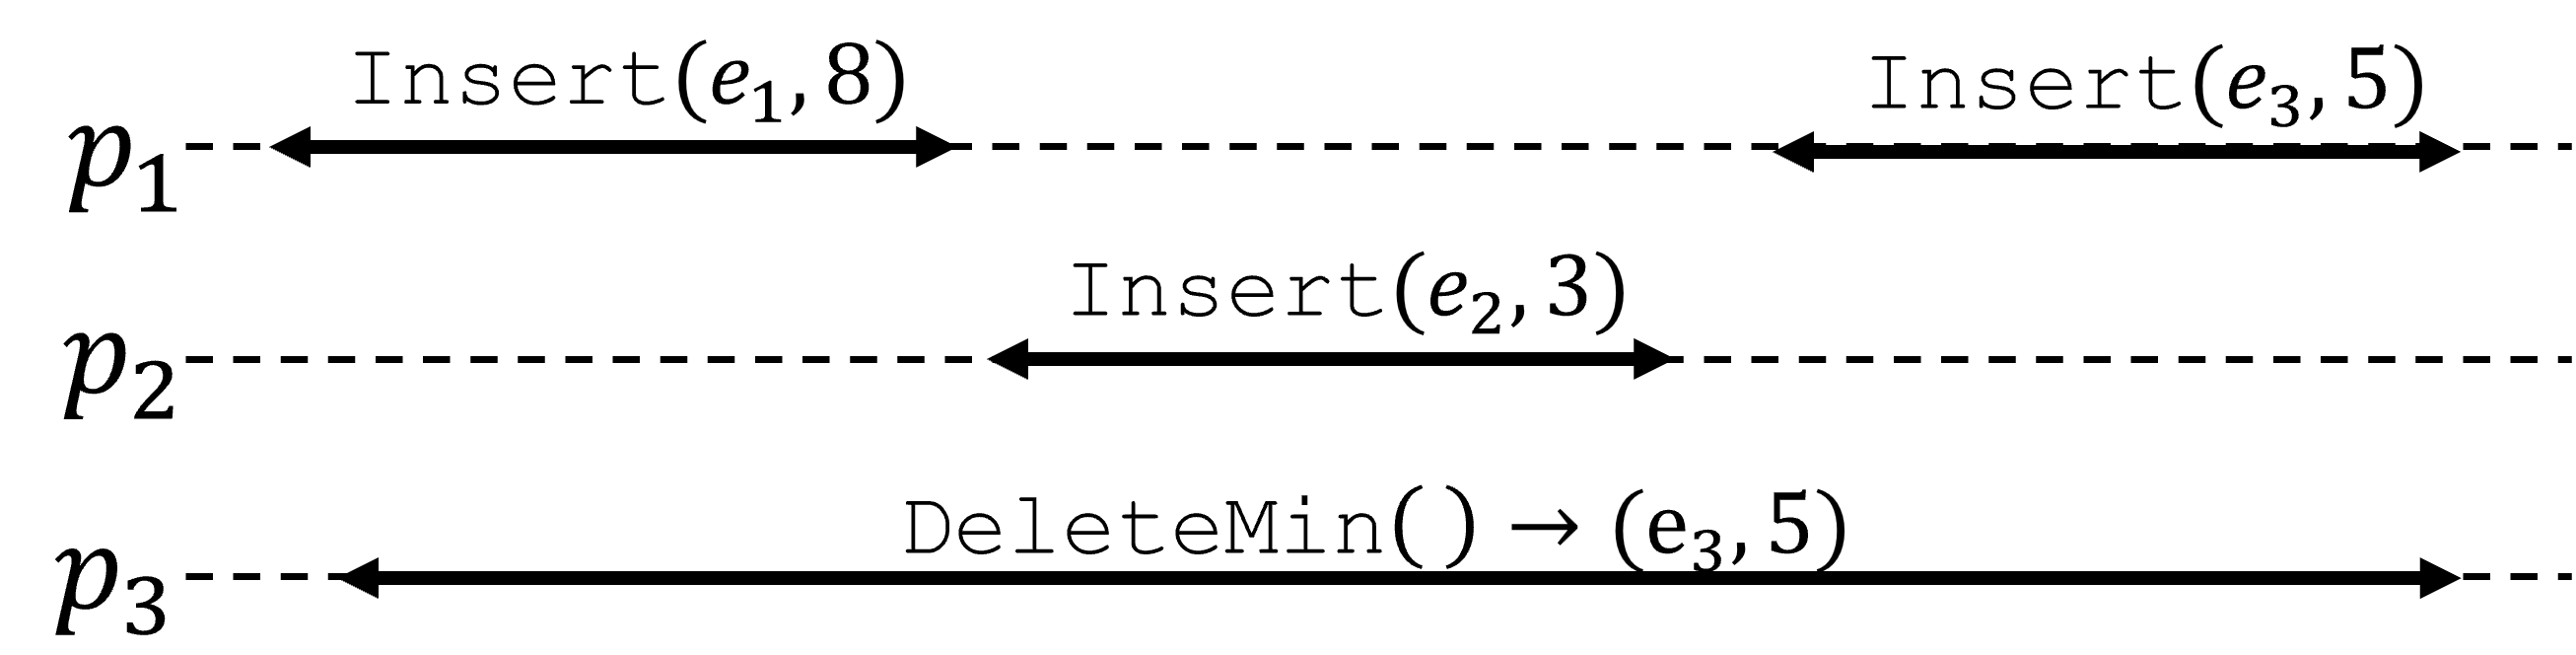
\includegraphics[width=0.4\textwidth]{graphics/ivl/PQIVLandSC.png}
  \caption{A possible concurrent history of a PQ that is both IVL and SC but not linearizable. The SC property requires that the remove be of some previously inserted element, and the IVL property requires that the element have a priority bound between $8$ and $3$.}
  \label{ivl-fig:SC-IVL-and-SC}
\end{figure}
